% Source of the figure chain-link.pdf (a chain link with its positive and negative path).
% Compile with pdfLaTeX; the PDF is included in the manuscript at its natural size.
\documentclass[tikz,border=1pt]{standalone}
\usepackage[T1]{fontenc}
\usepackage{stix}
\pdfinfoomitdate=1 \pdftrailerid{} \pdfsuppressptexinfo=-1
\definecolor{threadred}{RGB}{200,40,40}
\begin{document}
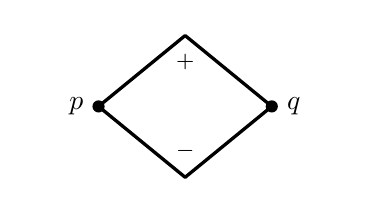
\begin{tikzpicture}[x=1cm, y=1cm,
    chain/.style={line width=1.2pt, line cap=round, line join=round},
    thread/.style={line width=0.8pt, line cap=round},
    crossing/.style={line width=2.6pt, line cap=butt},
    lead/.style={thread, densely dashed}]
  % The upper path is the positive path, the lower path the negative path.
  \useasboundingbox (-0.5,-1.0) rectangle (3.5,1.0);
  \draw[chain] (0.4,0) -- (1.5,0.9) -- (2.6,0) -- (1.5,-0.9) -- cycle;
  \node at (1.5,0.56) {\footnotesize $+$};
  \node at (1.5,-0.56) {\footnotesize $-$};
  \fill (0.4,0) circle[radius=2.2pt] (2.6,0) circle[radius=2.2pt];
  \node[left=2pt] at (0.4,0) {$p$};
  \node[right=2pt] at (2.6,0) {$q$};
\end{tikzpicture}
\end{document}
